%
% lemniskate.tex
%
% (c) 2021 Prof Dr Andreas Müller, OST Ostschweizer Fachhochschule
%
\section{Lemniskatischer Sinus
\label{buch:elliptisch:section:lemniskate}}
\rhead{Lemniskatischer Sinus}
Historisch war der {\em lemniskatische Sinus} die erste ellptische
Funktion, die Gauss bereits als 19-jähriger untersucht, aber nicht 
veröffentlich hat.
In diesem Abschnitt soll die Verbindung zu den Jacobischen
elliptischen Funktionen hergestellt werden.

%
% Lemniskate
%
\subsection{Lemniskate
\label{buch:gemotrie:subsection:lemniskate}}
\begin{figure}
\centering
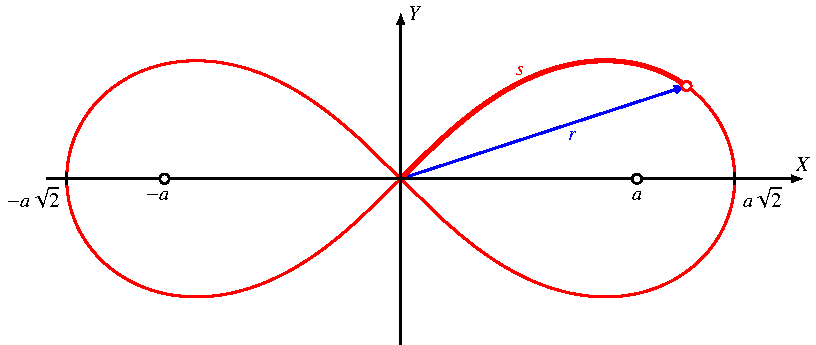
\includegraphics{chapters/110-elliptisch/images/lemniskate.pdf}
\caption{Bogenlänge und Radius der Lemniskate von Bernoulli.
\label{buch:elliptisch:fig:lemniskate}}
\end{figure}
Die {\em Lemniskate von Bernoulli} ist die Kurve vierten Grades
mit der Gleichung
\index{Lemniskate von Bernoulli}%
\begin{equation}
(X^2+Y^2)^2 = 2a^2(X^2-Y^2).
\label{buch:elliptisch:eqn:lemniskate}
\end{equation}
Sie ist in Abbildung~\ref{buch:elliptisch:fig:lemniskate}
dargestellt.
Der Fall $a=1/\sqrt{2}$ ist eine Kurve mit der Gleichung
\[
(x^2+y^2)^2 = x^2-y^2,
\]
wir nennen sie die {\em Standard-Lemniskate}.

\subsubsection{Scheitelpunkte}
Die beiden Scheitel der Lemniskate befinden sich bei $X_s=\pm a\sqrt{2}$.
Dividiert man die Gleichung der Lemniskate durch $X_s^2=4a^4$ entsteht 
\begin{equation}
\biggl(
\biggl(\frac{X}{a\sqrt{2}}\biggr)^2
+
\biggl(\frac{Y}{a\sqrt{2}}\biggr)^2
\biggr)^2
=
2\frac{a^2}{2a^2}\biggl(
\biggl(\frac{X}{a\sqrt{2}}\biggr)^2
-
\biggl(\frac{Y}{a\sqrt{2}}\biggr)^2
\biggr).
\qquad
\Leftrightarrow
\qquad
(x^2+y^2)^2 = x^2-y^2,
\label{buch:elliptisch:eqn:lemniskatenormiert}
\end{equation}
wobei wir $x=X/a\sqrt{2}$ und $y=Y/a\sqrt{2}$ gesetzt haben.
In dieser Normierung, der Standard-Lemniskaten, liegen die Scheitel
bei $\pm 1$.
Dies ist die Skalierung, die für die Definition des lemniskatischen
Sinus und Kosinus verwendet werden soll.

\subsubsection{Polarkoordinaten}
In Polarkoordinaten $x=r\cos\varphi$ und $y=r\sin\varphi$
gilt nach Einsetzen in \eqref{buch:elliptisch:eqn:lemniskatenormiert}
\begin{equation}
r^4
=
r^2(\cos^2\varphi-\sin^2\varphi)
=
r^2\cos2\varphi
\qquad\Rightarrow\qquad
r^2 = \cos 2\varphi
\label{buch:elliptisch:eqn:lemniskatepolar}
\end{equation}
als Darstellung der Lemniskate in Polardarstellung.
Sie gilt für Winkel $\varphi\in[-\frac{\pi}4,\frac{\pi}4]$ für das
rechte Blatt und $\varphi\in[\frac{3\pi}4,\frac{5\pi}4]$ für das linke
Blatt der Lemniskate.

%
% Schnitt eines Kegels mit einem Paraboloid
%
\subsubsection{Schnitt eines Kegels mit einem Paraboloid}
\begin{figure}
\center
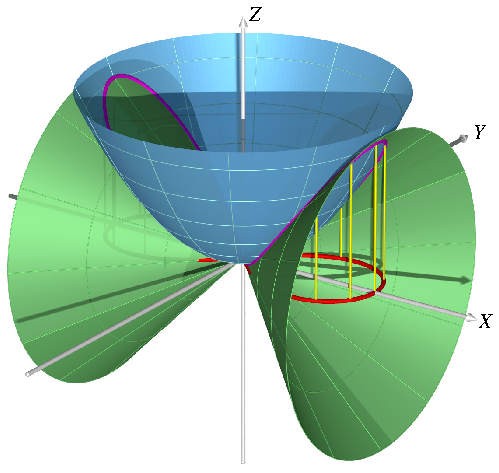
\includegraphics{chapters/110-elliptisch/images/kegelpara.pdf}
\caption{Leminiskate (rot) als Projektion (gelb) der Schnittkurve (pink)
eines geraden
Kreiskegels (grün) mit einem Rotationsparaboloid (hellblau).
\label{buch:elliptisch:lemniskate:kegelpara}}
\end{figure}%
\index{Kegel}%
\index{Paraboloid}%
Schreibt man in der Gleichung~\eqref{buch:elliptisch:eqn:lemniskate}
für die Klammer auf der rechten Seite $Z^2 = X^2 - Y^2$, dann wird die
Lemniskate die Projektion in die $X$-$Y$-Ebene der Schnittkurve der Flächen,
die durch die Gleichungen
\begin{equation}
X^2-Y^2 = Z^2
\qquad\text{und}\qquad
(X^2+Y^2) = R^2 = \sqrt{2}aZ
\label{buch:elliptisch:eqn:kegelparabolschnitt}
\end{equation}
beschrieben wird.
Die linke Gleichung in 
\eqref{buch:elliptisch:eqn:kegelparabolschnitt}
beschreibt einen geraden Kreiskegel, die rechte ist ein Rotationsparaboloid.
Die Schnittkurve ist in Abbildung~\ref{buch:elliptisch:lemniskate:kegelpara}
dargestellt.

\subsubsection{Schnitt eines Torus mit einer Ebene}
\begin{figure}
\centering
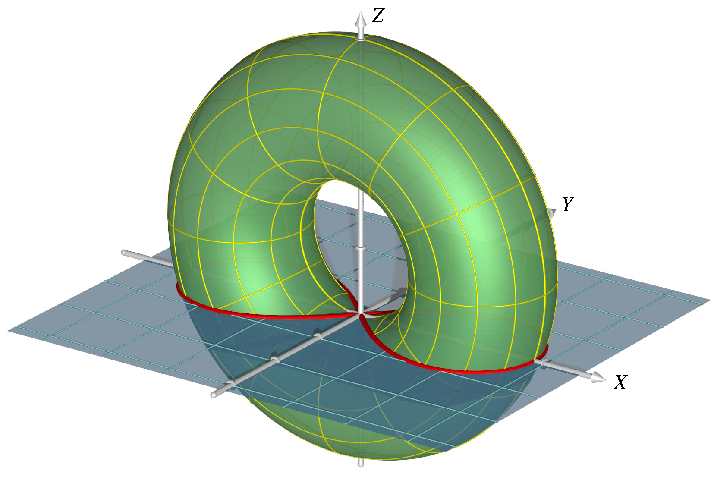
\includegraphics{chapters/110-elliptisch/images/torusschnitt.pdf}
\caption{Die Schnittkurve (rot) eines Torus (grün)
mit einer zur Torusachse parallelen Ebene (blau),
die den inneren Äquator des Torus berührt, ist eine Lemniskate.
\label{buch:elliptisch:lemniskate:torusschnitt}}
\end{figure}
\index{Torus}%
Schneidet man einen Torus mit einer Ebene, die zur Achse des Torus
parallel ist und den inneren Äquator des Torus berührt, wie in
Abbildung~\ref{buch:elliptisch:lemniskate:torusschnitt},
entsteht ebenfalls eine Lemniskate, wie in diesem Abschnitt nachgewiesen
werden soll.

Der in Abbildung~\ref{buch:elliptisch:lemniskate:torusschnitt}
dargestellte Torus mit den Radien $2$ und $1$ hat als Achse die
um eine Einheit in $Z$-Richtung verschobene $Y$-Achse und die
$X$-$Z$-Ebene als Äquatorebene.
Der Torus kann mit
\[
(u,v)
\mapsto
\begin{pmatrix}
(2+\cos u) \cos v    \\
   \sin u            \\
(2+\cos u) \sin v + 1
\end{pmatrix}
\]
parametrisiert werden, die $u$- und $v$-Koordinatenlinien sind 
in der Abbildung gelb eingezeichnet.
Die $v$-Koordinatenlinien sind Breitenkreise um die Achse des Torus.
Aus $u=0$ und $u=\pi$ ergeben sich die Äquatoren des Torus.

Die Gleichung $Z=0$ beschreibt eine achsparallele Ebene, die den
inneren Äquator berührt.
Die Schnittkurve erfüllt daher
\[
(2+\cos u)\sin v + 1 = 0,
\]
was wir auch als $2 +\cos u = -1/\sin v$ schreiben können.
Wir müssen nachprüfen, dass die Koordinaten
$X=(2+\cos u)\cos v$ und $Y=\sin u$ die Gleichung einer Lemniskate
erfüllen.

Zunächst können wir in der $X$-Koordinate den Klammerausdruck durch
$\sin v$ ausdrücken und erhalten
\begin{equation}
X
=
(2+\cos u) \cos v
=
-\frac{1}{\sin v}\cos v
=
-\frac{\cos v}{\sin v}
\qquad\Rightarrow\qquad
X^2
=
\frac{\cos^2v}{\sin^2 v}
=
\frac{1-\sin^2v}{\sin^2 v}.
\label{buch:elliptisch:lemniskate:Xsin}
\end{equation}
Auch die $Y$-Koordinaten können wir durch $v$ ausdrücken, 
nämlich
\begin{equation}
Y^2=\sin^2 u = 1-\cos^2 u
=
1-
\biggl(
\frac{1}{\sin v}
-2
\biggr)^2
=
\frac{-3\sin^2 v+4\sin v-1}{\sin^2 v}.
\label{buch:elliptisch:lemniskate:Ysin}
\end{equation}
Die Gleichungen
\eqref{buch:elliptisch:lemniskate:Xsin}
und
\eqref{buch:elliptisch:lemniskate:Ysin}
zeigen, dass man $X^2$ und $Y^2$ sogar einzig durch $\sin v$ 
parametrisieren kann.
Um die Ausdrücke etwas zu vereinfachen, schreiben wir $S=\sin v$
und erhalten zusammenfassend
\begin{equation}
\begin{aligned}
X^2
&=
\frac{1-S^2}{S^2}
\\
Y^2
&=
\frac{-3S^2+4S-1}{S^2}.
\end{aligned}
\end{equation}
Daraus kann man jetzt die Summen und Differenzen der Quadrate
berechnen, sie sind
\begin{equation}
\begin{aligned}
X^2+Y^2
&=
\frac{-4S^2+4S}{S^2}
=
\frac{4S(1-S)}{S^2}
=
\frac{4(1-S)}{S}
=
4\frac{1-S}{S}
\\
X^2-Y^2
&=
\frac{2-4S+2S^2}{S^2}
=
\frac{2(1-S)^2}{S^2}
=
2\biggl(\frac{1-S}{S}\biggr)^2.
\end{aligned}
\end{equation}
Die Berechnung des Quadrates von $X^2+Y^2$ ergibt die Gleichung
\[
(X^2+Y^2)^2
=
16
\biggl(\frac{1-S}{S}\biggr)^2
=
8 \cdot 2
\biggl(\frac{1-S}{S}\biggr)^2
=
2\cdot 2^2\cdot (X^2-Y^2).
\]
Sie ist eine Lemniskaten-Gleichung für $a=2$.

%
% Bogenlänge der Lemniskate
%
\subsection{Bogenlänge}
Die Funktionen
\begin{equation}
x(r) = \frac{r}{\sqrt{2}}\sqrt{1+r^2},
\quad
y(r) = \frac{r}{\sqrt{2}}\sqrt{1-r^2}
\label{buch:geometrie:eqn:lemniskateparam}
\end{equation}
erfüllen
\begin{align*}
x(r)^2-y(r)^2
&=
\frac{r^2(1+r^2)}{2}-\frac{r^2(1-r^2)}{2}
\\
&
=
r^4
=
(x(r)^2 + y(r)^2)^2,
\end{align*}
sie stellen also eine Parametrisierung der Standard-Lemniskate dar.

Mit Hilfe der Parametrisierung~\eqref{buch:geometrie:eqn:lemniskateparam}
kann man die Länge $s$ des in Abbildung~\ref{buch:elliptisch:fig:lemniskate}
dargestellten Bogens der Lemniskate berechnen.
Dazu benötigt man die Ableitungen nach $r$, die man mit der Produkt- und
Kettenregel berechnen kann:
\begin{align*}
\dot{x}(r)
&=
\frac{\sqrt{1+r^2}}{\sqrt{2}}
+
\frac{r^2}{\sqrt{2}\sqrt{1+r^2}}
&&\Rightarrow&
\dot{x}(r)^2
&=
\frac{1+r^2}{2} +r^2 + \frac{r^4}{2(1+r^2)}
\\
\dot{y}(r)
&=
\frac{\sqrt{1-r^2}}{\sqrt{2}}
-
\frac{r^2}{\sqrt{2}\sqrt{1-r^2}}
&&\Rightarrow&
\dot{y}(r)^2
&=
\frac{1-r^2}{2} -r^2 + \frac{r^4}{2(1-r^2)}.
\end{align*}
Die Summe der Quadrate ist
\begin{align*}
\dot{x}(r)^2 + \dot{y}(r)^2
&=
1 + r^4\frac{1-r^2+1+r^2}{2(1+r^2)(1-r^2)}
=
1+r^4\frac{2}{2(1-r^4)}
=
\frac{1-r^4+r^4}{1-r^4}
=
\frac1{1-r^4}.
\end{align*}
Durch Einsetzen in das Integral für die Bogenlänge bekommt man
\begin{equation}
s(r)
=
\int_0^r
\frac{1}{\sqrt{1-t^4}}\,dt.
\label{buch:elliptisch:eqn:lemniskatebogenlaenge}
\end{equation}

%
% Als elliptisches Integral
%
\subsection{Darstellung als elliptisches Integral}
Das unvollständige elliptische Integral erster Art mit Parameter
$k^2=-1$ oder $k=i$ ist
\[
K(r,i)
=
\int_0^x \frac{dt}{\sqrt{(1-t^2)(1-i^2 t^2)}}
=
\int_0^x \frac{dt}{\sqrt{(1-t^2)(1-(-1)t^2)}}
=
\int_0^x \frac{dt}{\sqrt{1-t^4}}
=
s(r).
\]
Der lemniskatische Sinus ist also eine Umkehrfunktion des
elliptischen Integrals erster Art für den speziellen Wert $i$ des
Parameters $k$.

Die Länge des rechten Blattes der Lemniskate wird mit $\varpi$ bezeichnet
und hat den numerischen Wert
\begin{equation}
\varpi
=
2\int_0^1\sqrt{\frac{1}{1-t^4}}\,dt
=
2.6220575542.
\label{buch:elliptisch:eqn:varpi}
\end{equation}
$\varpi$ ist auch als die {\em lemniskatische Konstante} bekannt.
\index{lemniskatische Konstante}%
Der Lemniskatenbogen zwischen dem Nullpunkt und $(1,0)$ hat die Länge
$\varpi/2$.

%
%  Bogenlängenparametrisierung
%
\subsection{Bogenlängenparametrisierung}
\begin{figure}
\centering
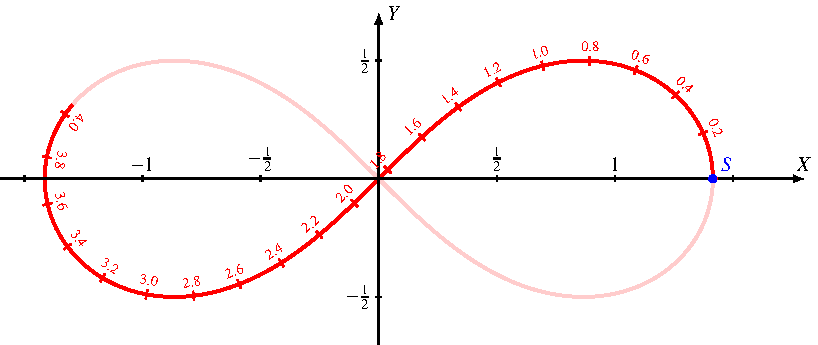
\includegraphics{chapters/110-elliptisch/images/lemnispara.pdf}
\caption{Parametrisierung der Lemniskate mit Jacobischen elliptischen
Funktion wie in \eqref{buch:elliptisch:lemniskate:bogeneqn}
\label{buch:elliptisch:lemniskate:bogenpara}}
\end{figure}
Die Lemniskate mit der Gleichung
\[
(X^2+Y^2)^2=2(X^2-Y^2)
\]
(der Fall $a=1$ in \eqref{buch:elliptisch:eqn:lemniskate})
kann mit Jacobischen elliptischen Funktionen
parametrisiert werden.
Dazu schreibt man
\begin{equation}
\left.
\begin{aligned}
X(t)
&=
\sqrt{2}\operatorname{cn}(t,k) \operatorname{dn}(t,k)
\\
Y(t)
&=
\phantom{\sqrt{2}}
\operatorname{cn}(t,k) \operatorname{sn}(t,k)
\end{aligned}
\quad\right\}
\qquad\text{mit $k=\displaystyle\frac{1}{\sqrt{2}}$}
\label{buch:elliptisch:lemniskate:bogeneqn}
\end{equation}
Abbildung~\ref{buch:elliptisch:lemniskate:bogenpara} zeigt die
Parametrisierung. 
Dem Parameterwert $t=0$ entspricht der Scheitelpunkt
$S=(\sqrt{2},0)$ der Lemniskate.

%
% Lemniskatengleichung
%
\subsubsection{Verfikation der Lemniskatengleichung}
Dass \eqref{buch:elliptisch:lemniskate:bogeneqn}
tatsächlich eine Parametrisierung ist kann nachgewiesen werden dadurch,
dass man die beiden Seiten der definierenden Gleichung der
Lemniskate berechnet.
Zunächst ist
\begin{align*}
X(t)^2
&=
2\operatorname{cn}(t,k)^2
\operatorname{dn}(t,k)^2
\\
Y(t)^2
&=
\operatorname{cn}(t,k)^2
\operatorname{sn}(t,k)^2
\\
X(t)^2+Y(t)^2
&=
2\operatorname{cn}(t,k)^2
\bigl(
\underbrace{
\operatorname{dn}(t,k)^2
+{\textstyle\frac12}
\operatorname{sn}(t,k)^2
}_{\displaystyle =1}
\bigr)
%\\
%&
=
2\operatorname{cn}(t,k)^2
\\
X(t)^2-Y(t)^2
&=
\operatorname{cn}(t,k)^2
\bigl(
2\operatorname{dn}(t,k)^2 - \operatorname{sn}(t,k)^2
\bigr)
\\
&=
\operatorname{cn}(t,k)^2
\bigl(
2\bigl({\textstyle\frac12}+{\textstyle\frac12}\operatorname{cn}(t,k)^2\bigr)
-
\bigl(1-\operatorname{cn}(t,k)^2\bigr)
\bigr)
\\
&=
2\operatorname{cn}(t,k)^4
\\
\Rightarrow\qquad
(X(t)^2+Y(t)^2)^2
&=
4\operatorname{cn}(t,k)^4
=
2(X(t)^2-Y(t)^2).
\end{align*}

%
% Berechnung der Bogenlänge
%
\subsubsection{Berechnung der Bogenlänge}
Wir zeigen jetzt, dass dies tatsächlich eine Bogenlängenparametrisierung
der Lemniskate ist.
Dazu berechnen wir die Ableitungen
\begin{align*}
\dot{X}(t)
&=
\sqrt{2}\operatorname{cn}'(t,k)\operatorname{dn}(t,k)
+
\sqrt{2}\operatorname{cn}(t,k)\operatorname{dn}'(t,k)
\\
&=
-\sqrt{2}\operatorname{sn}(t,k)\operatorname{dn}(t,k)^2
-\frac12\sqrt{2}\operatorname{sn}(t,k)\operatorname{cn}(t,k)^2
\\
&=
-\sqrt{2}\operatorname{sn}(t,k)\bigl(
1-{\textstyle\frac12}\operatorname{sn}(t,k)^2
+{\textstyle\frac12}-{\textstyle\frac12}\operatorname{sn}(t,k)^2
\bigr)
\\
&=
\sqrt{2}\operatorname{sn}(t,k)
\bigl(
{\textstyle \frac32}-\operatorname{sn}(t,k)^2
\bigr)
\\
\dot{X}(t)^2
&=
2\operatorname{sn}(t,k)^2
\bigl(
{\textstyle \frac32}-\operatorname{sn}(t,k)^2
\bigr)^2
\\
&=
{\textstyle\frac{9}{2}}\operatorname{sn}(t,k)^2
-
6\operatorname{sn}(t,k)^4
+2\operatorname{sn}(t,k)^6
\\
\dot{Y}(t)
&=
\operatorname{cn}'(t,k)\operatorname{sn}(t,k)
+
\operatorname{cn}(t,k)\operatorname{sn}'(t,k)
\\
&=
-\operatorname{sn}(t,k)^2
\operatorname{dn}(t,k)
+\operatorname{cn}(t,k)^2
\operatorname{dn}(t,k)
\\
&=
\operatorname{dn}(t,k)\bigl(1-2\operatorname{sn}(t,k)^2\bigr)
\\
\dot{Y}(t)^2
&=
\bigl(1-{\textstyle\frac12}\operatorname{sn}(t,k)^2\bigr)
\bigl(1-2\operatorname|{sn}(t,k)^2\bigr)^2
\\
&=
1-{\textstyle\frac{9}{2}}\operatorname{sn}(t,k)^2
+6\operatorname{sn}(t,k)^4
-2\operatorname{sn}(t,k)^6
\\
\dot{X}(t)^2 + \dot{Y}(t)^2
&=
1.
\end{align*}
Dies bedeutet, dass die Bogenlänge zwischen den Parameterwerten $0$ und $t$
\[
\int_0^t
\sqrt{\dot{X}(\tau)^2 + \dot{Y}(\tau)^2}
\,d\tau
=
\int_0^s\,d\tau
=
t,
\]
der Parameter $t$ ist also ein Bogenlängenparameter.

%
% Bogenlängenparametrisierung der Standard-Lemniskate
%
\subsubsection{Bogenlängenparametrisierung der Standard-Lemniskate}
Die mit dem Faktor $1/\sqrt{2}$ skalierte Standard-Lemniskate mit der
Gleichung
\[
(x^2+y^2)^2 = x^2-y^2
\]
hat daher eine Bogenlängenparametrisierung mit
\begin{equation}
\left.
\begin{aligned}
x(t)
&=
\phantom{\frac{1}{\sqrt{2}}}
\operatorname{cn}(\sqrt{2}t,k)\operatorname{dn}(\sqrt{2}t,k)
\\
y(t)
&=
\frac{1}{\sqrt{2}}
\operatorname{cn}(\sqrt{2}t,k)\operatorname{sn}(\sqrt{2}t,k)
\end{aligned}
\quad
\right\}
\qquad
\text{mit $\displaystyle k=\frac{1}{\sqrt{2}}$}
\label{buch:elliptisch:lemniskate:bogenlaenge}
\end{equation}
Der Punkt $t=0$ entspricht dem Scheitelpunkt $S=(1,0)$ der Lemniskate.
Der Parameter misst also die Bogenlänge entlang der Lemniskate ausgehend
vom Scheitel.

%
% der lemniskatische Sinus und Kosinus
%
\subsection{Der lemniskatische Sinus und Kosinus}
Der Sinus berechnet die Gegenkathete zu einer gegebenen Bogenlänge des
Kreises, er ist die Umkehrfunktion der Funktion, die der Gegenkathete
die Bogenlänge zuordnet.
Daher ist es naheliegend, die Umkehrfunktion von $s(r)$ in 
\eqref{buch:elliptisch:eqn:lemniskatebogenlaenge}
den {\em lemniskatischen Sinus} zu nennen mit der Bezeichnung
\index{lemniskatischer Sinus}%
\index{Sinus, lemniskatischer}%
$r=r(s)=\operatorname{sl} s$.
\index{komplementäre Bogenlänge}

%
% die komplementäre Bogenlänge
%
\subsubsection{Die komplementäre Bogenlänge}
Der Kosinus ist der Sinus des komplementären Winkels.
Auch für die lemniskatische Bogenlänge $s(r)$ lässt sich eine
komplementäre Bogenlänge $t$ definieren, nämlich die Bogenlänge
zwischen dem Punkt $(x(r), y(r))$ und dem Scheitelpunkt $S=(1,0)$.
Dies ist der Parameter der Parametrisierung
\eqref{buch:elliptisch:lemniskate:bogenlaenge}
des vorangegangenen Abschnittes.
Die Bogenlänge zwischen $O=(0,0)$ und $S=(1,0)$ wurde in
\eqref{buch:elliptisch:eqn:varpi} bereits bereichnet,
sie ist $\varpi/2$.
Damit folgt für die beiden Parameter $s$ und $t$ die Beziehung
$t = \varpi/2 - s$.

\subsubsection{Der lemniskatische Kosinus}
\begin{figure}
\centering
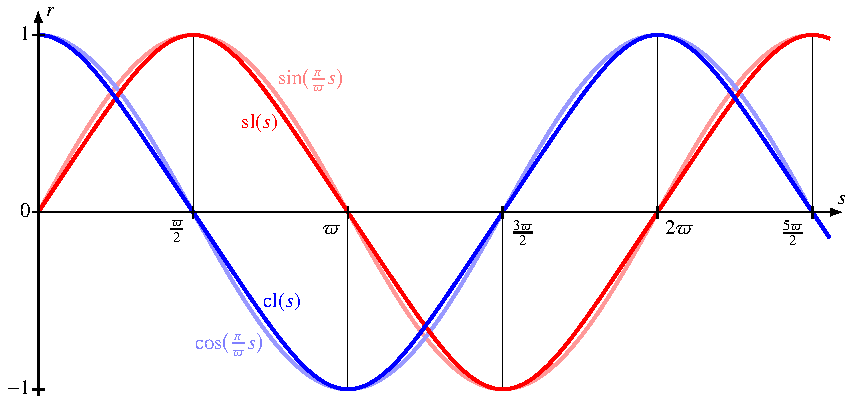
\includegraphics[width=\textwidth]{chapters/110-elliptisch/images/slcl.pdf}
\caption{
Lemniskatischer Sinus und Kosinus sowie Sinus und Kosinus
mit derart skaliertem Argument, dass die Funktionen die
gleichen Nullstellen haben.
\label{buch:elliptisch:figure:slcl}}
\end{figure}
Der {\em lemniskatische Kosinus} ist daher
$\operatorname{cl}(s) = \operatorname{sl}(\varpi/2-s)$.
Graphen des lemniskatische Sinus und Kosinus sind in
Abbildung~\ref{buch:elliptisch:figure:slcl} dargestellt.

Die Parametrisierung~\eqref{buch:elliptisch:lemniskate:bogenlaenge}
ist eine Bogenlängenparametrisierung der Standard-Lemniskate.
Man kann sie verwenden, um $r(t)$ zu berechnen.
Es ist
\[
r(t)^2
=
x(t)^2 + y(t)^2
=
\operatorname{cn}(\sqrt{2}t,k)^2
\biggl(
\operatorname{dn}(\sqrt{2}t,k)^2
+
\frac12
\operatorname{sn}(\sqrt{2}t,k)^2
\biggr)
=
\operatorname{cn}(\sqrt{2}t,k)^2.
\]
Die Wurzel ist
\[
r(t)
=
\operatorname{cn}(\sqrt{2}t,{\textstyle\frac{1}{\sqrt{2}}})
.
\]
Der lemniskatische Sinus wurde aber in Abhängigkeit von
$s=\varpi/2-t$ mittels
\[
\operatorname{sl}s
=
r(s)
=
\operatorname{cn}(\sqrt{2}(\varpi/2-s),k)^2
\]
definiert.
Der lemniskatische Kosinus ist definiert als der lemniskatische Sinus
\index{lemniskatischer Kosinus}%
\index{Kosinus, lemniskatischer}%
der komplementären Bogenlänge, also
\[
\operatorname{cl}(s)
=
\operatorname{sl}(\varpi/2-s)
=
\operatorname{cn}(\sqrt{2}s,k)^2.
\]
Die Funktion $\operatorname{sl}(s)$ und $\operatorname{cl}(s)$ sind
in Abbildung~\ref{buch:elliptisch:figure:slcl} dargestellt.
Sie sind beide $2\varpi$-periodisch.
Die Abbildung zeigt ausserdem die Funktionen $\sin (\pi s/\varpi)$
und $\cos(\pi s/\varpi)$, die ebenfalls $2\varpi$-periodisch sind.


